\documentclass{article}
\usepackage{graphicx}
\usepackage{hyperref}


\begin{document}
\title{Aufgabe: Logische Uhren und happens-before}
\maketitle

\section{Einführung}
In diesem Dokument beschäftigen wir uns mit einer Sequenz von Nachrichten, die zwischen vier Knoten in einem Netzwerk ausgetauscht werden. Die Sequenz ist im Diagramm~\ref{fig:sequenzdiagramm} dargestellt:

\begin{figure}[h]
\centering
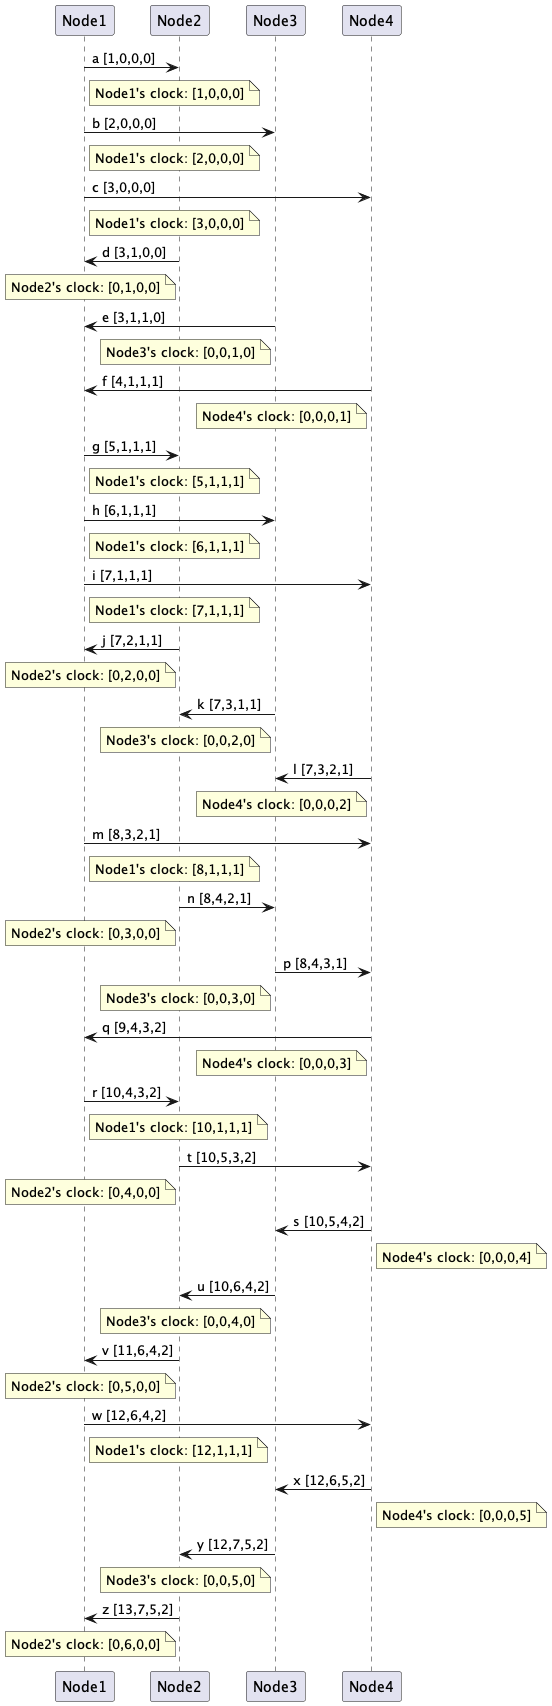
\includegraphics[width=0.65\textwidth]{../../fig/uml/clock_exam_concurrent.png}
\caption{Sequenzdiagramm der Nachrichten}
\label{fig:sequenzdiagramm}
\end{figure}

\section{Aufgaben}

\subsection{Aufgabe 1}
Beschreiben Sie die Nachrichtensequenz von Node1 zu den anderen Knoten. Geben Sie die Reihenfolge der Nachrichten an.

\subsection{Aufgabe 2}
Welche Nachrichten sind konkurrierend? Was bedeutet das in diesem Kontext?

\subsection{Aufgabe 3}
Beschreiben Sie den Nachrichtenfluss, der mit der Nachricht `j` beginnt und mit der Nachricht `t` endet. Welche Knoten sind beteiligt?

\subsection{Aufgabe 4}
Erweitern Sie das Sequenzdiagramm um zwei weitere Knoten, die Nachrichten mit den Knoten 1 bis 4 austauschen. Was ändert sich in Bezug auf die Komplexität des Netzwerks?

\subsection{Aufgabe 5}
Schreiben Sie ein kurzes Programm in einer Programmiersprache Ihrer Wahl, das diesen Nachrichtenaustausch simuliert. Was sind die Herausforderungen bei der Simulation dieser Sequenz?

\end{document}
